\documentclass{standalone}
\usepackage{tikz}
\usetikzlibrary{shapes,arrows,positioning,fit,decorations.pathmorphing}

\begin{document}
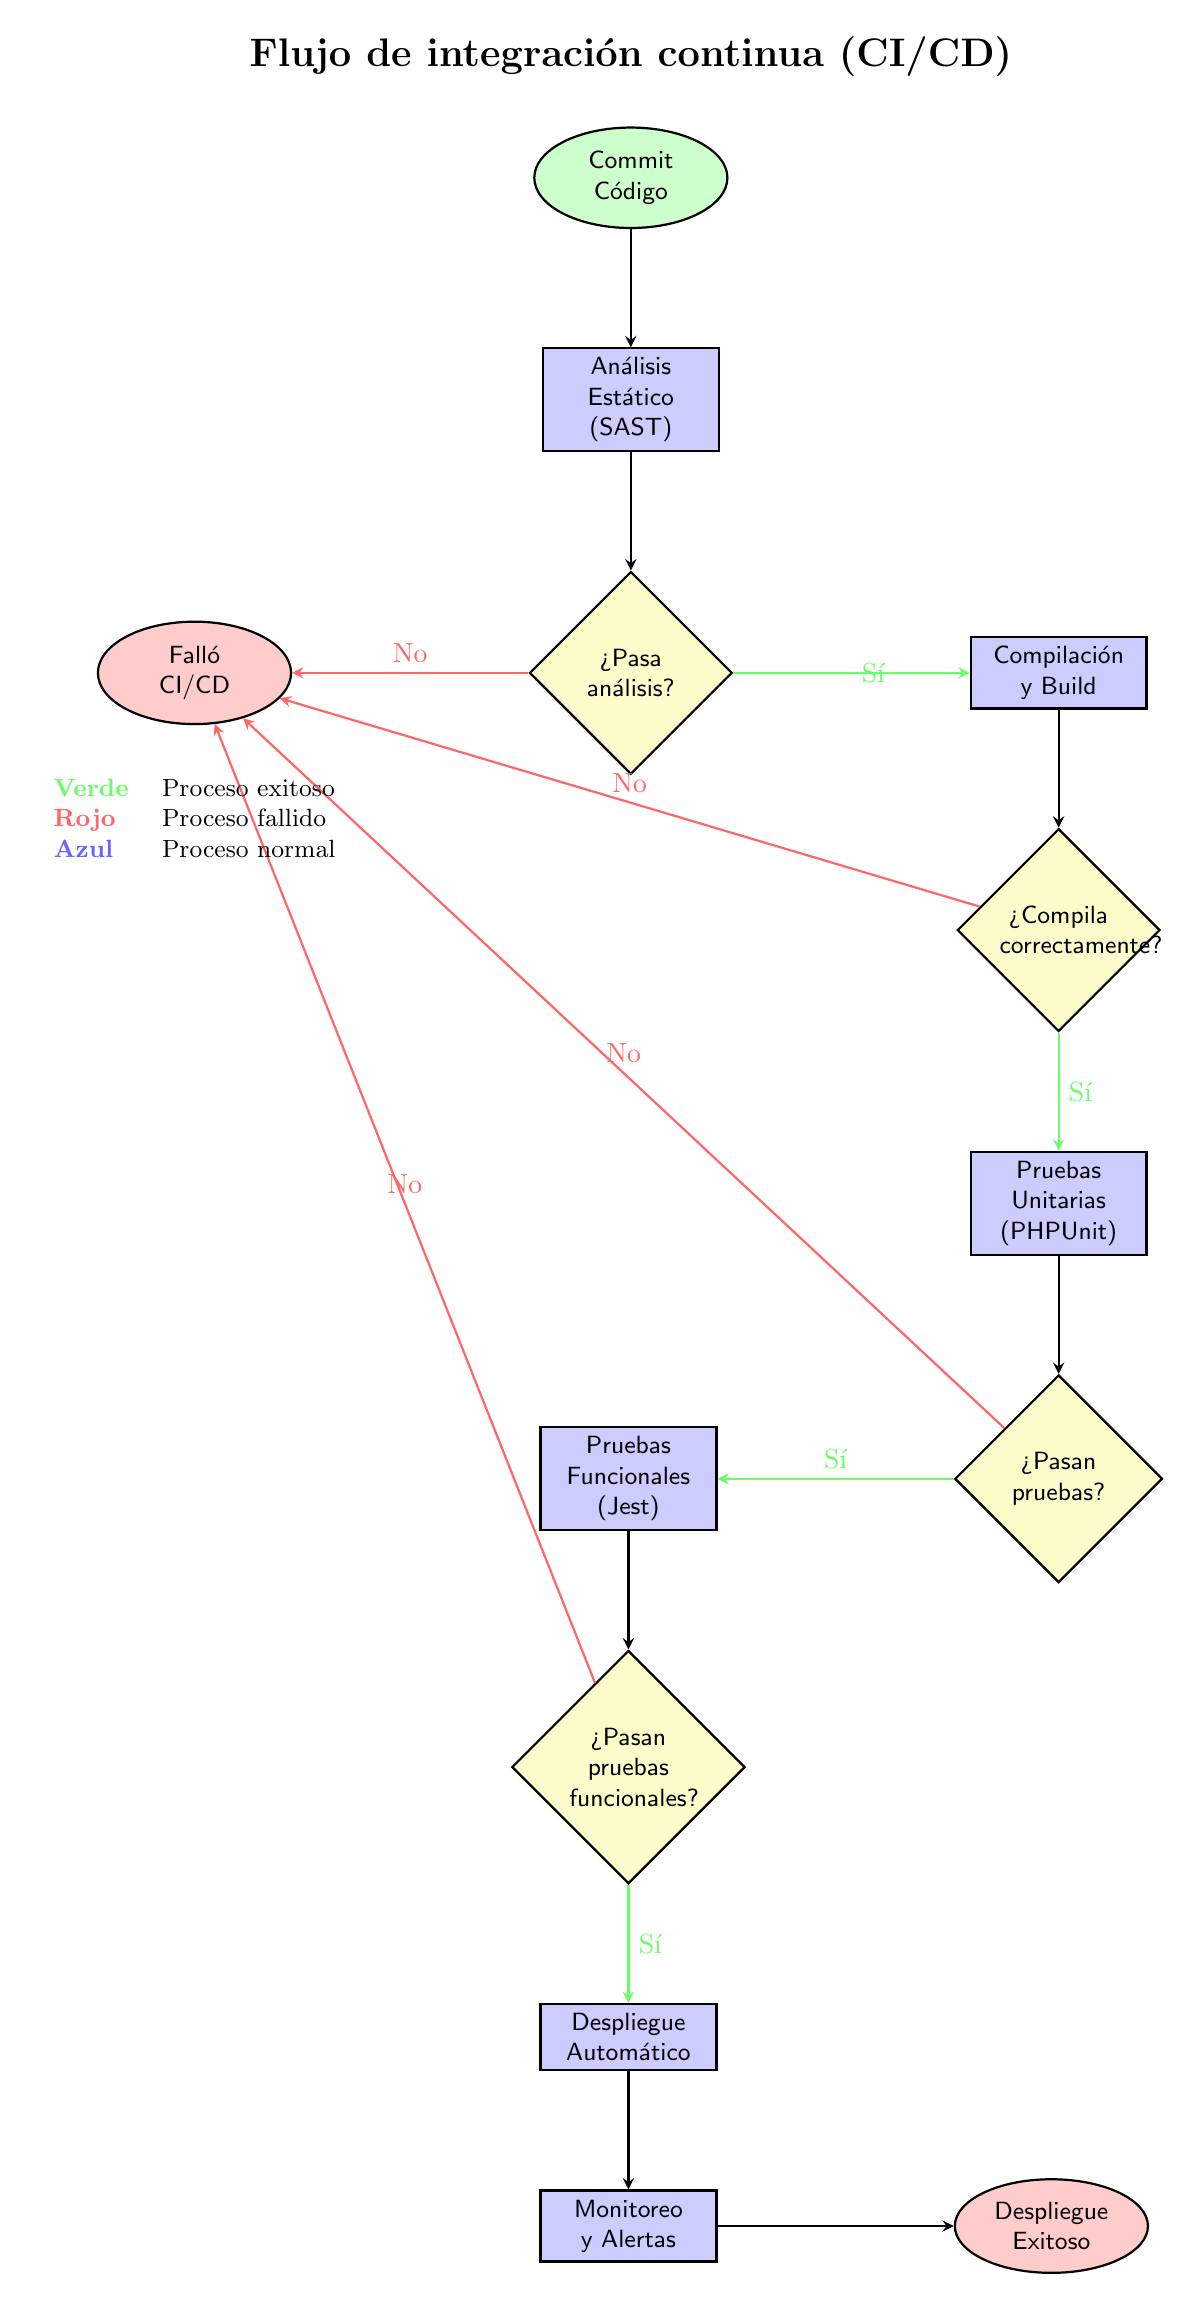
\begin{tikzpicture}[
    node distance=1.5cm,
    auto,
    thick,
    process/.style={rectangle,fill=blue!20,draw,font=\sffamily\small,text width=2cm,text centered},
    decision/.style={diamond,fill=yellow!20,draw,font=\sffamily\small,text width=1.5cm,text centered},
    start/.style={ellipse,fill=green!20,draw,font=\sffamily\small,text width=1.5cm,text centered},
    end/.style={ellipse,fill=red!20,draw,font=\sffamily\small,text width=1.5cm,text centered},
    arrow/.style={->,>=stealth,thick},
    success/.style={arrow,green!60},
    failure/.style={arrow,red!60}
]

% Inicio
\node[start] (start) {Commit\\Código};

% Proceso 1: Análisis estático
\node[process, below=of start] (static) {Análisis\\Estático\\(SAST)};

% Decisión 1: ¿Pasa análisis?
\node[decision, below=of static] (check1) {¿Pasa\\análisis?};

% Proceso 2: Compilación
\node[process, right=3cm of check1] (compile) {Compilación\\y Build};

% Decisión 2: ¿Compila?
\node[decision, below=of compile] (check2) {¿Compila\\correctamente?};

% Proceso 3: Pruebas unitarias
\node[process, below=of check2] (unit) {Pruebas\\Unitarias\\(PHPUnit)};

% Decisión 3: ¿Pasan pruebas?
\node[decision, below=of unit] (check3) {¿Pasan\\pruebas?};

% Proceso 4: Pruebas funcionales
\node[process, left=3cm of check3] (func) {Pruebas\\Funcionales\\(Jest)};

% Decisión 4: ¿Pasan pruebas funcionales?
\node[decision, below=of func] (check4) {¿Pasan\\pruebas\\funcionales?};

% Proceso 5: Despliegue
\node[process, below=of check4] (deploy) {Despliegue\\Automático};

% Proceso 6: Monitoreo
\node[process, below=of deploy] (monitor) {Monitoreo\\y Alertas};

% Fin exitoso
\node[end, right=3cm of monitor] (success) {Despliegue\\Exitoso};

% Fin fallido
\node[end, left=3cm of check1] (failure) {Falló\\CI/CD};

% Conexiones principales
\draw[arrow] (start) -- (static);
\draw[arrow] (static) -- (check1);
\draw[success] (check1) -- node[right] {Sí} (compile);
\draw[failure] (check1) -- node[above] {No} (failure);

\draw[arrow] (compile) -- (check2);
\draw[success] (check2) -- node[right] {Sí} (unit);
\draw[failure] (check2) -- node[above] {No} (failure);

\draw[arrow] (unit) -- (check3);
\draw[success] (check3) -- node[above] {Sí} (func);
\draw[failure] (check3) -- node[above] {No} (failure);

\draw[arrow] (func) -- (check4);
\draw[success] (check4) -- node[right] {Sí} (deploy);
\draw[failure] (check4) -- node[above] {No} (failure);

\draw[arrow] (deploy) -- (monitor);
\draw[arrow] (monitor) -- (success);

% Título
\node[above=0.5cm of start, font=\Large\bfseries] {Flujo de integración continua (CI/CD)};

% Leyenda
\node[below=0.5cm of failure, font=\small] {
    \begin{tabular}{ll}
        \textcolor{green!60}{\textbf{Verde}} & Proceso exitoso \\
        \textcolor{red!60}{\textbf{Rojo}} & Proceso fallido \\
        \textcolor{blue!60}{\textbf{Azul}} & Proceso normal
    \end{tabular}
};

\end{tikzpicture}
\end{document}
